\documentclass[tikz,border=10pt]{standalone}
% No extra libraries needed
\begin{document}
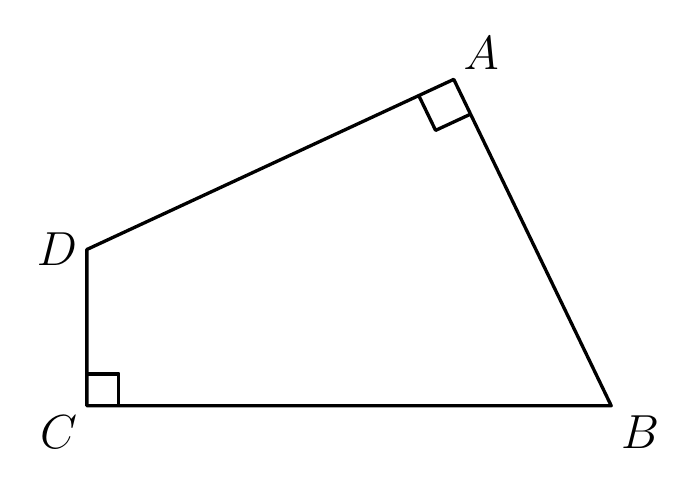
\begin{tikzpicture}[line join=round]
  % Vertices (pixel coords converted with s = 0.021108, y flipped, centre (230,164))
  \coordinate (A) at (1.283,2.077);
  \coordinate (B) at (3.283,-2.069);
  \coordinate (C) at (-3.377,-2.069);
  \coordinate (D) at (-3.377,-0.084);

  % Right-angle mark corners
  % at C (between CB and CD)
  \coordinate (c1) at (-2.971,-2.069);
  \coordinate (c2) at (-2.971,-1.663);
  \coordinate (c3) at (-3.377,-1.663);
  % at A (between AD and AB)
  \coordinate (a1) at (0.839,1.870);
  \coordinate (a2) at (1.052,1.429);
  \coordinate (a3) at (1.496,1.635);

  % Quadrilateral ABCD, solid black
  \draw[line width=1.2pt, black] (A) -- (B) -- (C) -- (D) -- cycle;

  % Right-angle markers (one per vertex)
  \draw[line width=1.2pt, black] (c1) -- (c2) -- (c3);
  \draw[line width=1.2pt, black] (a1) -- (a2) -- (a3);

  % Vertex labels
  \node[above right] at (A) {\fontsize{17}{20.4}\selectfont $A$};
  \node[below right] at (B) {\fontsize{17}{20.4}\selectfont $B$};
  \node[below left] at (C) {\fontsize{17}{20.4}\selectfont $C$};
  \node[left] at (D) {\fontsize{17}{20.4}\selectfont $D$};
\end{tikzpicture}
\end{document}